%! TEX root = 'main.tex'
\section{Background}
\label{sec:background}


The term Industrial Control System (ICS) describes different control systems and associated instrumentation, including the devices, systems, networks, and controls used to operate and automate industrial processes. Supervisory Control and Data Acquisition (SCADA) systems and Distributed Control Systems (DCS) are the most common ICS. The ICS connects sensors and actuators that interact with the physical systems (e.g., power grid) with the cyber components such as networks and servers. Local operations are often controlled by so-called Field Devices that receive supervisory commands from remote stations. Whether it has remote communication components, the controller field devices are categorized as Programmable Logic Controller (PLC) and Remote Terminal Unit (RTU). They are used in both DCS and SCADA systems as a control component of an overall system. 

\textbf{\textit{PLC}}. PLCs consist of a processor, I/O modules, a power supply, and other specialized addon modules. The I/O modules of PLCs interact with the physical world, gathering digital inputs from sensors, switch, or a thermometer. The processor servers the PLC's brain executes pre-programmed ladder logic based on the inputs and gives operation signals through the output module. That said, it is not easy to tell the difference between a PLC and an embedded system. Usually, they both use a microcontroller as the processor. PLCs are designed and rigorously tested to withstand operating in an industrial environment where they may be exposed to vibration and noise. 

With an embedded system solution, the choice of the microcontroller is various. Moreover, each system has its own specialized circuit board design around it. On the contrary, several major PLC vendors dominate the market so that only numerous models are widely used, and particular programming tool-chain such as ladder logic is used. Therefore, from the attacker's perspective, anyone who purchases the same-model PLC will have the exact hardware and software environment as the target system.

The PLC has a firmware acting as the real-time operating system. It also provides library routines to operate on various I/O devices such as I2C and SPI. These routines may reside at fixed addresses of the ROM. The firmware loads the control logic, such as a compile ladder logic binary at bootstrap or each update initiated from the remote operator.

The ladder logic programs are executed repeatedly in fixed intervals, called scan cycles. When the logic calls the firmware routines to toggle an output pin, it is carried out by setting/clearing a memory bit, which is the MMIO address corresponding to output pins, thus to the sockets of the I/O module. PLC usually has LEDs at the front panel to indicate the inputs and output pins' current status.


\textbf{\textit{JTAG.}} JTAG interface named after Joint Test Action Group, is a industry standard port for IC testing. This is necessary because of the growing complexity of integrated circuits makes the design verification tends to be more and more difficult.

The JTAG interface use very few pins (TDI, TDO, TMS and TCK) to talk to test access port(TAP) which implements a state machine and a set of registers to further connect more circuit components, from which it can access memory bus and more debug facilities, as shown in ~\autoref{fig:jtagsm}. The two major register of TAP are Instruction Register(IR) and Data Register(DR). They work in a serial mode in which they accepts/sends out bit stream through the four former mentioned JTAG pins. The IR register contains the command to be executed, DR contains shift-in data or the command's result. JTAG is just a way to read/write data to different registers/components that connected to the system. It's early applications targeted board level testing, diagnosis and fault isolation. Nowadays JTAG is used as the primary way of accessing sub-blocks of integrated circuits, making it the most common way to debug embedded system. In this project, the PLC we work with use ARM cortex-m3 based microcontroller, ARM Cortex-M series  contains CoreSight Technology which is a power debug model. The CoreSight can't be operated through either JTAG or SWD(Serial Wire Debug) interface.

\begin{figure}[th]
	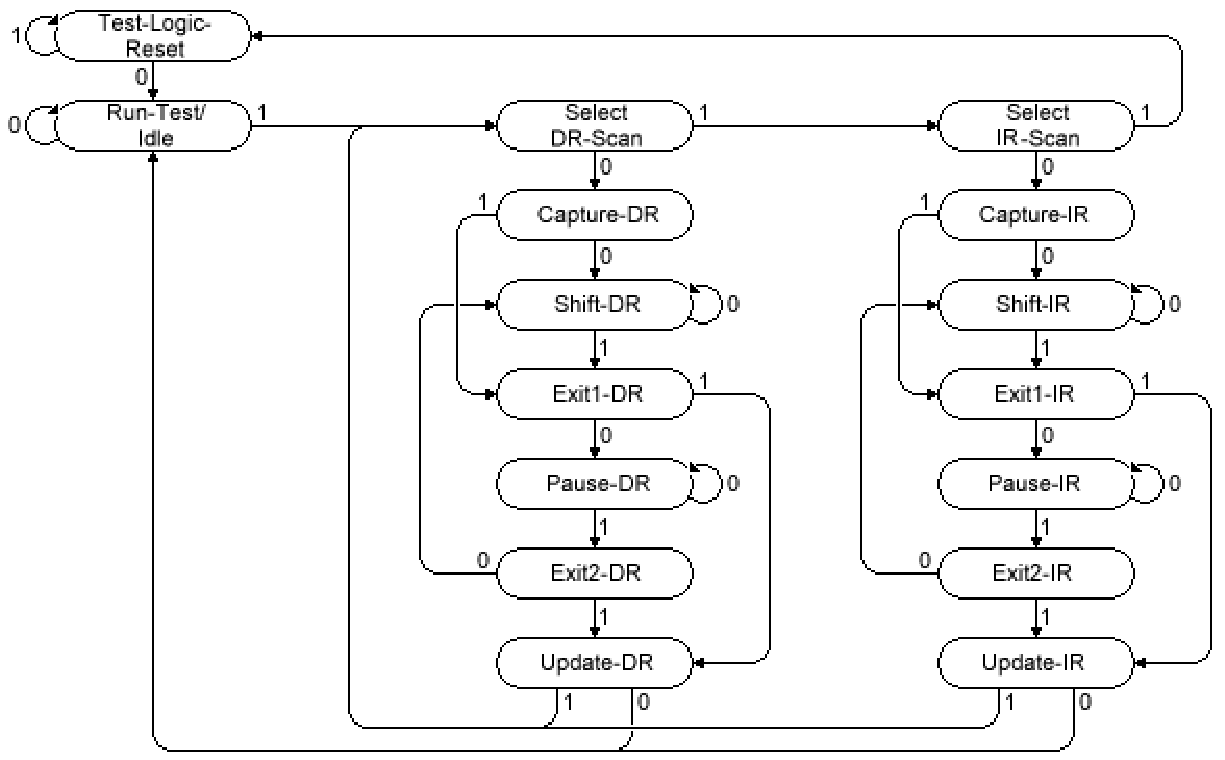
\includegraphics[width=0.47\textwidth]{figures/jtagsm}
	\centering
	\caption{JTAG TAP state machine.}
	\label{fig:jtagsm}
\end{figure}


On ARM Cortex-M series microcontroller has build on a Debug Access Port(DAP) which is comprised of a Debug Port(DP) and several Access Ports(AP). DP manages the connection to an external debugger. APs access on-chip system resources. DAPBUS connects the DP to one or more APs. The APs provide non-invasive access to APB bus though APB-AP,  and to other legacy-configured debug components using JTAG-AP. In our project, we access system memory and memory-mapped IO through AHB-AP. Because of this comprehensive debug ability that ARM provide, our hardware implant can fully control the system by connects to the JTAG pins.

On the real-time microcontroller board, we found JTAG solder joints, as shown in~\autoref{fig:board_jtag}. It supports both JTAG and SWD (Serial Wire Debug\cite{ashfieldserial}) interfaces. In this paper, we choose to use JTAG interface. But if you use the SWD interface, some of the pins will be reused as SWD pins. 

\begin{figure}[th]
	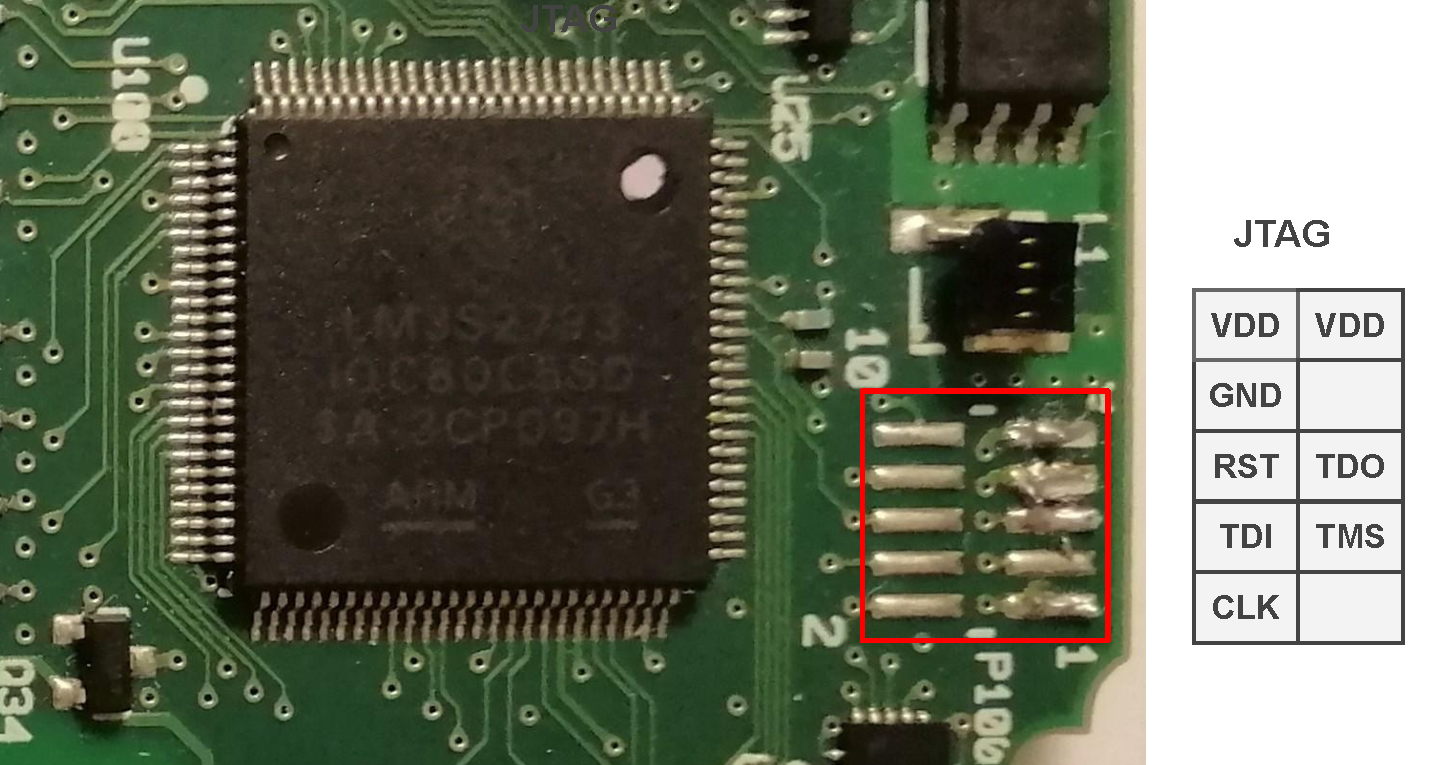
\includegraphics[width=0.47\textwidth]{figures/board_jtag}
	\centering
	\caption{JTAG Interface on the Real-time Microcontroller Board}
	\label{fig:board_jtag}
\end{figure}

The JTAG specification allows for several devices to be connected to a single interface in a daisy chain configuration. In this case, we found that there is only one microcontroller connected.

Because we want to implement JTAG debugging functionality on a very small device, in order to be able to fit into the PLC case. Currently we choose Teensy 3.2 development board. For smaller PCB boards, smaller chips are required, such as an 8-bit microcontroller system, which typically has very limited on-chip memory. So we choose to implement the JTAG driver ourselves, instead of choosing an open source project, such as OpenOCD\cite{hogl2006open}. The code for implementing JTAG debugging with Teensy 3.2 development board has been uploaded to github\footnote{https://github.com/whensungoesdown/teensyi\_jtag}. It only needs to modify 4 GPIO pins, so it can be easily ported to other devices.
